% https://github.com/PetarV-/TikZ/blob/master/Coordinate%20systems/coordinate_systems.tex
\documentclass[crop, tikz, border=10pt]{standalone}
\usepackage{tikz}

\usetikzlibrary{calc}

\definecolor{olivegreen}{rgb}{0,0.6,0}

\begin{document}
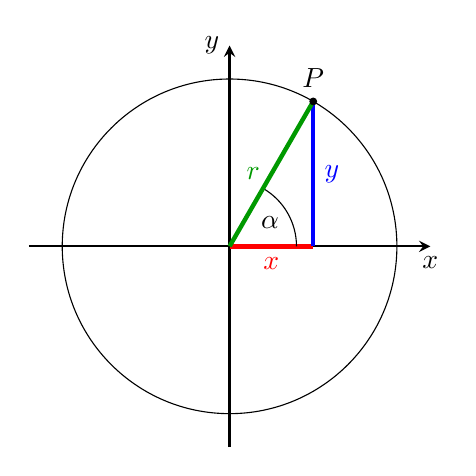
\begin{tikzpicture}[scale=0.85]
	% Axis
	\draw[thick,-stealth,black] (-3,0)--(3,0) coordinate (A) node[below] {$x$}; % x axis
	\draw[thick,-stealth,black] (0,-3)--(0,3) node[left] {$y$}; % y axis
	\draw[black,thin] (0,0) circle (2.5cm);
	
	\draw[ultra thick,red] (0,0) -- (60:2.5cm |- 0,0) node[midway,below] {$x$}; % UpOn y axis

	\draw (1,0) arc (0:60:1) node at ($(60/2:0.7)$) {$\alpha$};
	\draw[ultra thick, blue] (60:2.5cm) -- (60:2.5cm |- 0,0) node[midway,right] {$y$}; % vertical line

	\draw[ultra thick,olivegreen,rotate=60] (0,0) -- node [left] {$r$} (2.5,0) coordinate (B); 
    
	\draw[xshift=-1cm] (B) node[circle,fill,inner sep=1pt,label=above:$P$](e){};
\end{tikzpicture}
\end{document}